% TUBA 4-pillar summary: one-glance overview suitable for the GitHub
% landing page. One full-width figure per species so the atlas/skull
% overlays are readable. Built with the shared compactarticle.cls.
\documentclass{compactarticle}

\usepackage{graphicx}
\usepackage{booktabs}
\usepackage{enumitem}
\usepackage{xcolor}
\usepackage{float}
\usepackage{url}
\usepackage{listings}

\graphicspath{{./}{../mouse/figures/}{../macaque/figures/}{../human/figures/}{../rat/figures/}}

\begin{document}
\fancyhead[R]{\small\itshape TUBA -- four-pillar overview}

\articletype{Overview}

\title{TUBA: transcranial ultrasound brain atlas \\
       \large four species, one pipeline}

\author{Gianmarco F Pinton}

\affil{Joint Department of Biomedical Engineering, University of North
       Carolina at Chapel Hill and North Carolina State University}

\email{gia@email.unc.edu}

\begin{abstract}
TUBA is an open-source Python pipeline that registers a species-specific
skull microCT to its canonical brain atlas, producing the (geometry,
intensity, atlas-label) tuple needed for transcranial ultrasound simulation. Four species pillars are operational --- mouse,
macaque, human, and rat --- and share the same core primitives
(\texttt{tuba.core.\{frame, downsample, align, cavity, registration,
slab, placement\}}). Each pillar's calibration is documented in its
own validation report (\texttt{docs/<species>/manuscript.pdf}).
\end{abstract}

\section{Per-species snapshot}

\begin{table}[H]
\centering\small
\begin{tabular}{lllll}
\toprule
\textbf{Pillar} & \textbf{Skull source} & \textbf{Native pitch} & \textbf{Brain atlas} & \textbf{Cavity vol.} \\
\midrule
Mouse   & Maga 4K microCT (UW)~\cite{maga-uw}            & 6.13\,$\mu$m  & Allen CCFv3~\cite{allen-ccfv3}                          & 0.45\,mL \\
Macaque & AMNH M-87264~\cite{copes2016}                   & 60.6\,$\mu$m  & NMT v2 + CHARM~\cite{nmt-v2} + SARM~\cite{sarm} + D99~\cite{d99}   & 88\,mL   \\
Human   & Halle Zenodo~\cite{kirchner2022}                & 125\,$\mu$m   & MNI152~\cite{fonov2011} + Harvard-Oxford~\cite{harvardoxford} + Schaefer~\cite{schaefer2018} & 1300\,mL \\
Rat     & DigiMorph TMM M-2272~\cite{digimorph-rat}       & 29.6\,$\mu$m  & WHS SD v4.01~\cite{whs-papp-2014, whs-v4}              & 2.39\,mL \\
\bottomrule
\end{tabular}
\end{table}

% ---- Mouse ----
\begin{figure}[H]
\centering

\includegraphics[width=\textwidth,keepaspectratio]{registration_qc.pdf}
\caption{\textbf{Mouse} --- Allen CCFv3 atlas (warm overlay) +
         668-region annotation (categorical palette) warped onto
         the Maga 4K dry-skull microCT, with the extracted
         endocranial cavity (cyan contour, 0.45\,mL). ANTs SyN.}
\end{figure}

% ---- Macaque ----
\begin{figure}[H]
\centering
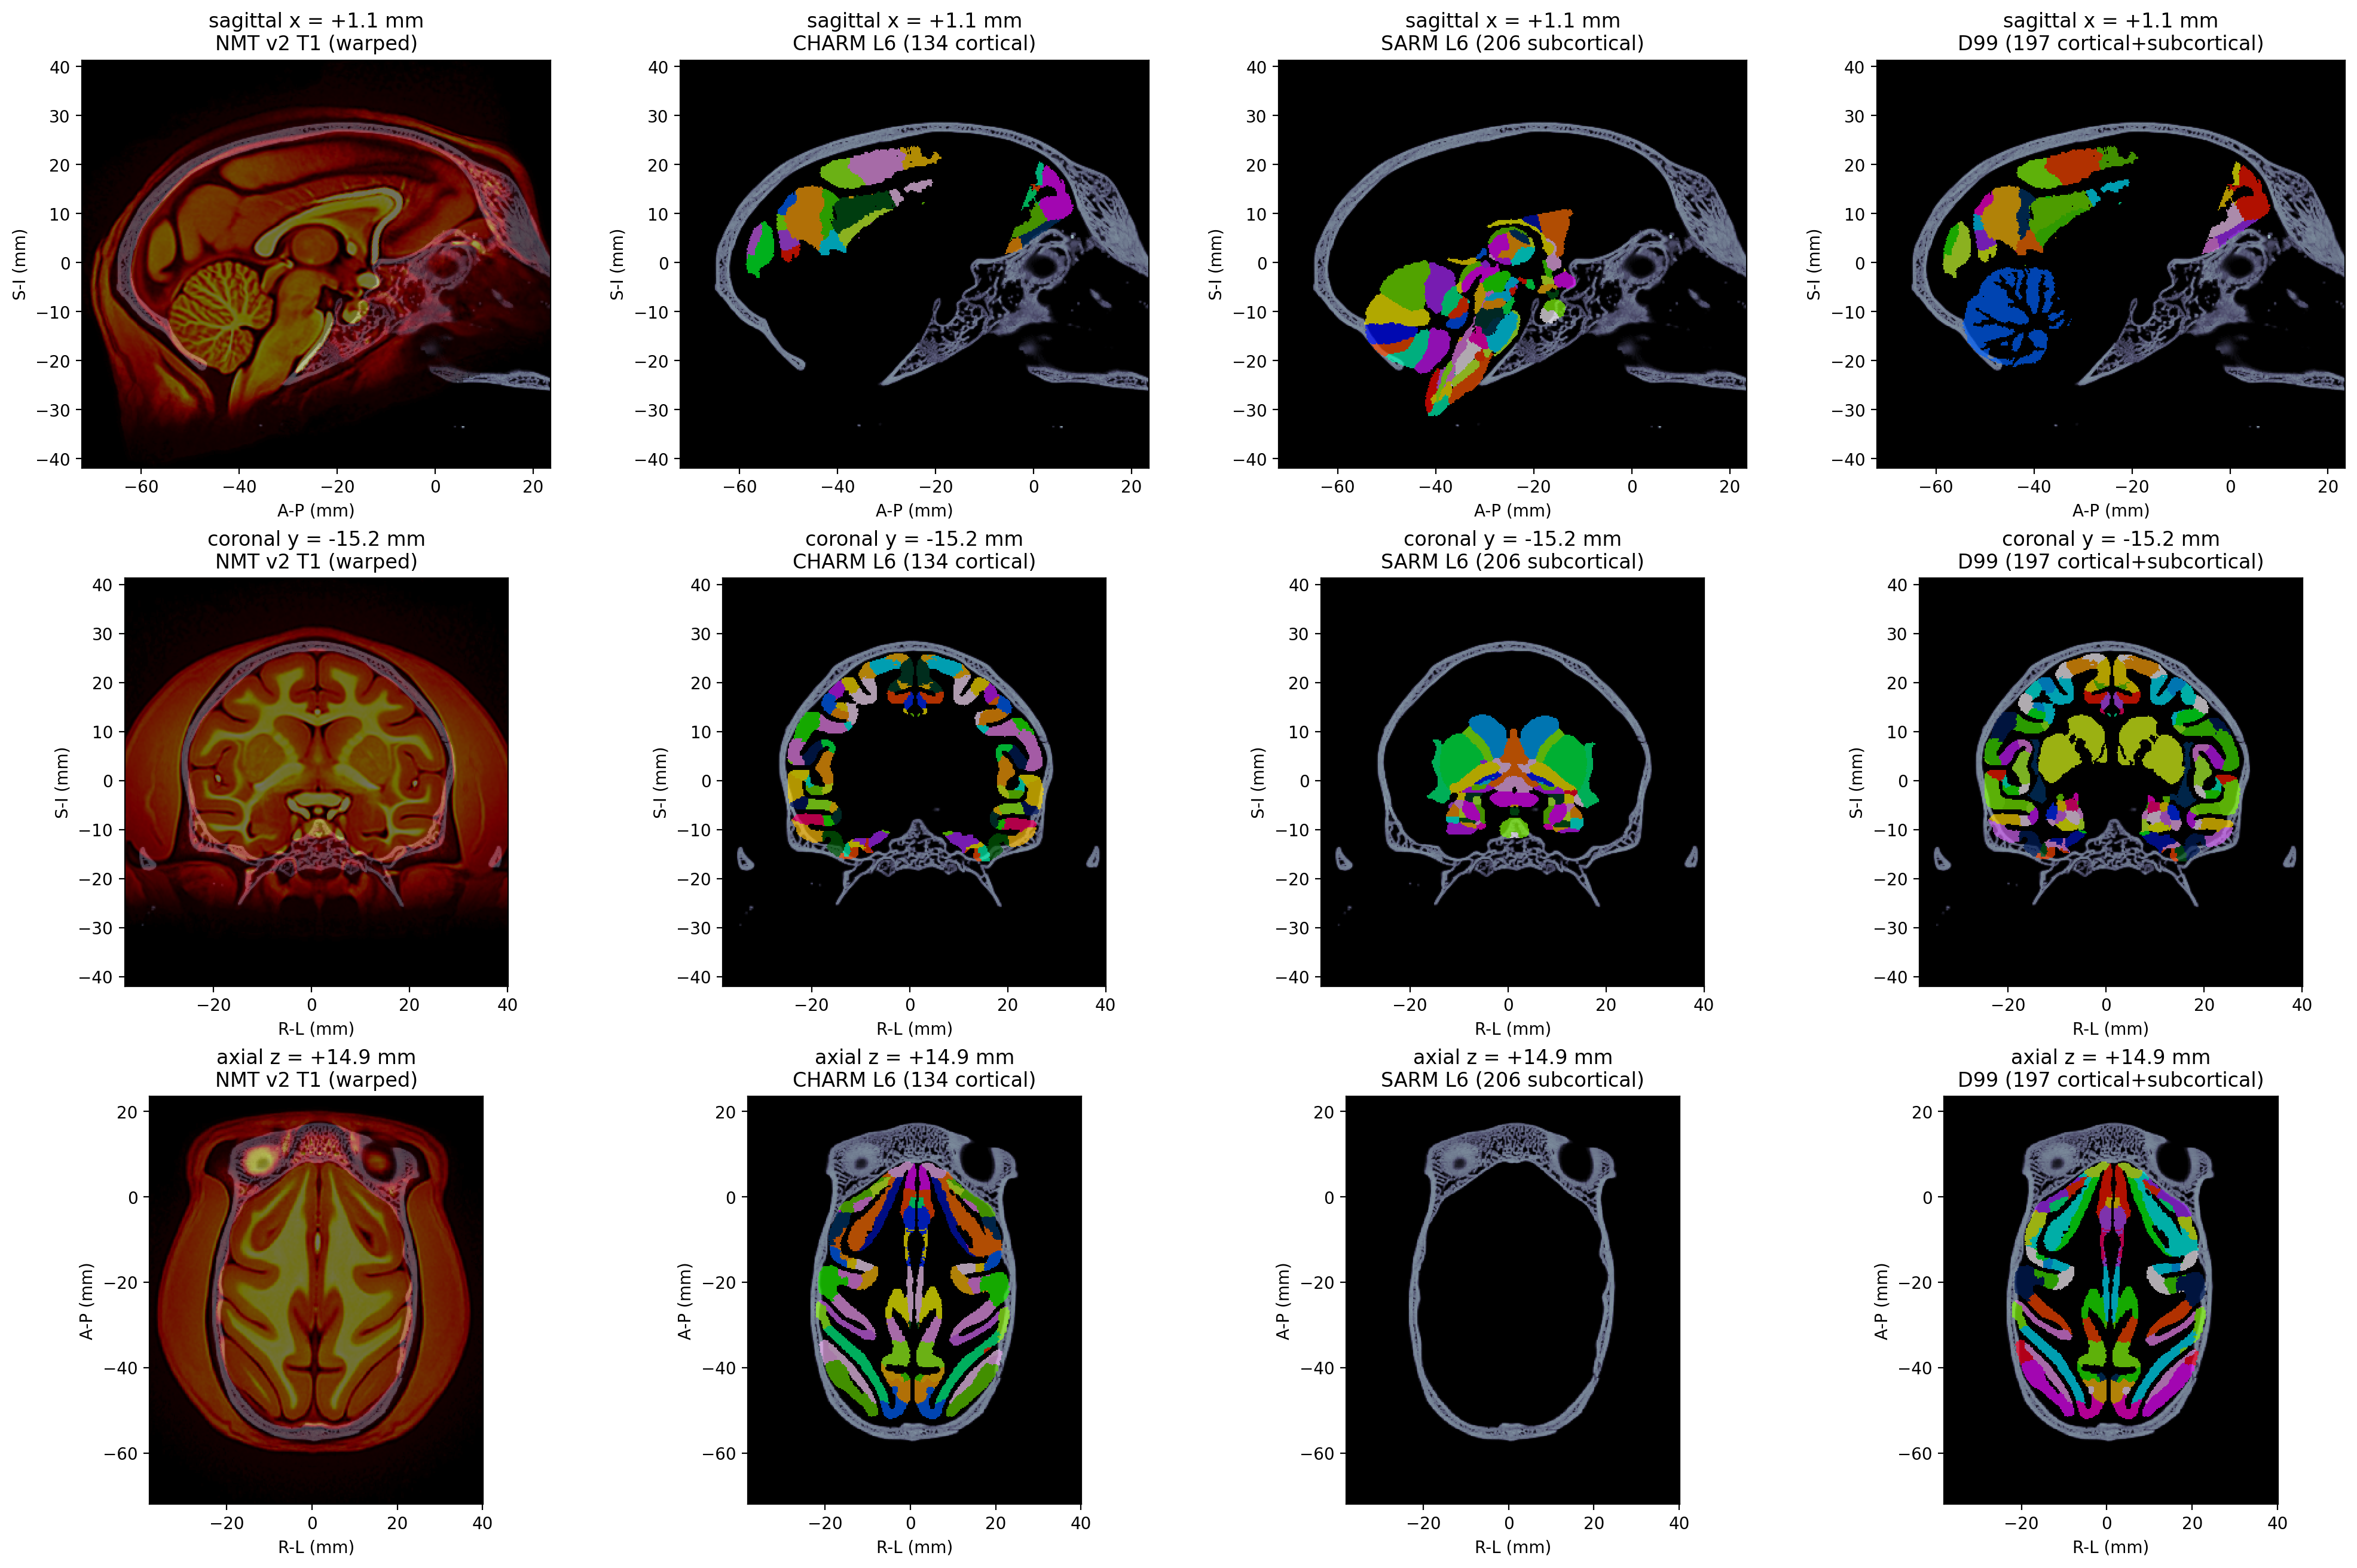
\includegraphics[width=\textwidth,keepaspectratio]{nmt_atlases_in_macaque.png}
\caption{\textbf{Macaque} --- NMT v2 T1 template + CHARM cortical
         parcellation warped into AMNH M-87264 skull space via ANTs
         Affine (no SyN). Endocranial cavity 88\,mL.}
\end{figure}

% ---- Human ----
\begin{figure}[H]
\centering
\includegraphics[width=\textwidth,keepaspectratio]{fig4_warped_atlases_on_halle.png}
\caption{\textbf{Human} --- Harvard-Oxford 117 + Schaefer 400 +
         Schaefer 1000 atlas labels warped onto the Halle Zenodo
         dry-skull CT (Kirchner 2022) via ANTs SyN through MNI152.
         Endocranial cavity ${\sim}1300$\,mL.}
\end{figure}

% ---- Rat ----
\begin{figure}[H]
\centering

\includegraphics[width=\textwidth,keepaspectratio]{registration_qc.png}
\caption{\textbf{Rat} --- WHS v4.01 SD rat atlas (T2$^*$ template
         + 222-structure annotation) warped onto the DigiMorph
         TMM M-2272 skull via ANTs Affine (cavity in cyan, 2.39\,mL).}
\end{figure}

\section{Pipeline at a glance}

Each pillar runs the same logical sequence; species differences are
encoded in the \texttt{tuba.species.<name>} module's constants.

\begin{enumerate}[leftmargin=*,itemsep=0pt]
\item \textbf{Fetch} skull volume + atlas via the
      \texttt{src/tuba/data/fetch\_*.py} fetchers (provenance pinned
      in \texttt{sources.toml} with SHA-256 checksums).
\item \textbf{Orient + downsample} into RAS world frame
      (\texttt{tuba.core.frame}, \texttt{tuba.core.downsample}).
\item \textbf{PCA pre-align} when required (mouse, macaque); skipped
      for human and rat after the row/col swap.
\item \textbf{Extract cavity}: mouse uses hysteresis-threshold
      (\texttt{tuba.core.cavity.extract\_cavity}); macaque and rat use
      the bone-shell builder (\texttt{tuba.core.cavity.bone\_shell\_cavity});
      human uses raycast outer-bone surface.
\item \textbf{Register} the species atlas onto the cavity (Affine
      for macaque, rat; SyN for mouse, human).
\item \textbf{Load slab}: \texttt{tuba.species.<name>.load\_slab()}
      returns $(c, \rho, dz, \mathrm{frame})$ for the FDTD /
      angular-spectrum driver.
\end{enumerate}

\section{Code}

A pillar load is one call:

\begin{lstlisting}[basicstyle=\small\ttfamily,
                   backgroundcolor=\color{black!5},
                   frame=single,framerule=0pt]
from tuba.species import mouse, macaque, human, rat

c, rho, dz, frame = rat.load_slab()  # or mouse / macaque / human
\end{lstlisting}

Per-pillar validation reports (with the full calibration trail,
intensity histograms, cavity QC, and atlas-warp QC) live at
\texttt{docs/<species>/manuscript.pdf}. The combined codebase is at
\url{https://github.com/pinton-lab/tuba}.

% =============================================================================
% Each reference title is hyperlinked to a Google Scholar lookup so
% the PDF reader can jump straight to the canonical landing page.
\providecommand{\gs}[2]{\href{https://scholar.google.com/scholar?q=#1}{#2}}

\begin{thebibliography}{99}

% ---- Skull microCT sources ----
\bibitem{maga-uw} M.~Maga and collaborators,
  \emph{\href{https://faculty.washington.edu/maga/SCRI_MicroCT/}{Sample
  microCT data from the SCRI Bone and Skeletal Mechanics Lab}},
  University of Washington.

\bibitem{copes2016} L.\,E.~Copes, L.\,M.~Lucas, J.\,O.~Thostenson,
  H.\,E.~Hoekstra, and D.\,M.~Boyer,
  \gs{10.1038/sdata.2016.1}{``A collection of non-human primate
  computed tomography scans housed in MorphoSource, a repository
  for 3D data''},
  \emph{Sci.\ Data} {\bf 3}, 160001 (2016).
  doi:10.1038/sdata.2016.1.

\bibitem{kirchner2022} T.~Kirchner,
  \gs{Kirchner+2022+micro-CT+human+skull+Zenodo+6108435}{``A micro-CT
  of a human skull''}, Zenodo (2022).
  doi:10.5281/zenodo.6108435.

\bibitem{digimorph-rat} T.\,B.~Rowe and J.\,A.~Maisano,
  \emph{\href{https://digimorph.org/specimens/Rattus_norvegicus/}{Rattus
  norvegicus} (TMM M-2272)}, Digital Morphology Library, University
  of Texas at Austin.

% ---- Brain atlases ----
\bibitem{allen-ccfv3} Q.~Wang, S.-L.~Ding, Y.~Li, J.~Royall,
  D.~Feng, P.~Lesnar, N.~Graddis, M.~Naeemi, B.~Facer, A.~Ho
  \emph{et al.},
  \gs{10.1016/j.cell.2020.04.007}{``The Allen Mouse Brain Common
  Coordinate Framework: A 3D Reference Atlas''},
  \emph{Cell} {\bf 181}(4), 936--953.e20 (2020).
  doi:10.1016/j.cell.2020.04.007.

\bibitem{nmt-v2} B.~Jung, P.\,A.~Taylor, J.~Seidlitz, C.~Sponheim,
  P.~Perkins, L.\,G.~Ungerleider, D.~Glen, and A.~Messinger,
  \gs{10.1016/j.neuroimage.2021.117997}{``A comprehensive macaque
  fMRI pipeline and hierarchical atlas''},
  \emph{NeuroImage} {\bf 235}, 117997 (2021).
  doi:10.1016/j.neuroimage.2021.117997.

\bibitem{sarm} R.~Hartig, D.~Glen, B.~Jung, N.\,K.~Logothetis,
  G.~Paxinos, E.\,A.~Garza-Villarreal, A.~Messinger, and C.~Evrard,
  \gs{10.1016/j.neuroimage.2021.117996}{``The Subcortical Atlas of
  the Rhesus Macaque (SARM) for neuroimaging''},
  \emph{NeuroImage} {\bf 235}, 117996 (2021).
  doi:10.1016/j.neuroimage.2021.117996.

\bibitem{d99} K.\,S.~Saleem and N.~Logothetis,
  \emph{\gs{Saleem+Logothetis+Combined+MRI+Histology+Atlas+Rhesus+Monkey+Brain+Stereotaxic+Coordinates}{A
  Combined MRI and Histology Atlas of the Rhesus Monkey Brain in
  Stereotaxic Coordinates}}, 2nd ed., Academic Press (2012).

\bibitem{fonov2011} V.~Fonov, A.\,C.~Evans, K.~Botteron,
  C.\,R.~Almli, R.\,C.~McKinstry, D.\,L.~Collins, and the
  Brain Development Cooperative Group,
  \gs{Fonov+2011+Unbiased+average+age-appropriate+atlases+pediatric+studies+NeuroImage}{``Unbiased
  average age-appropriate atlases for pediatric studies''},
  \emph{NeuroImage} {\bf 54}(1), 313--327 (2011).

\bibitem{harvardoxford} R.\,S.~Desikan, F.~S\'egonne, B.~Fischl,
  B.\,T.~Quinn, \emph{et al.},
  \gs{10.1016/j.neuroimage.2006.01.021}{``An automated labeling
  system for subdividing the human cerebral cortex on MRI scans
  into gyral based regions of interest''} (basis of the
  Harvard--Oxford cortical atlas distributed with FSL),
  \emph{NeuroImage} {\bf 31}(3), 968--980 (2006).
  doi:10.1016/j.neuroimage.2006.01.021.

\bibitem{schaefer2018} A.~Schaefer, R.~Kong, E.\,M.~Gordon,
  T.\,O.~Laumann, X.-N.~Zuo, A.\,J.~Holmes, S.\,B.~Eickhoff, and
  B.\,T.\,T.~Yeo,
  \gs{Schaefer+2018+Local-global+parcellation+human+cerebral+cortex+intrinsic+functional+connectivity+MRI}{``Local-global
  parcellation of the human cerebral cortex from intrinsic
  functional connectivity MRI''},
  \emph{Cerebral Cortex} {\bf 28}(9), 3095--3114 (2018).

\bibitem{whs-papp-2014} E.\,A.~Papp, T.\,B.~Leergaard, E.~Calabrese,
  G.\,A.~Johnson, and J.\,G.~Bjaalie,
  \gs{10.1016/j.neuroimage.2014.04.001}{``Waxholm Space atlas of the
  Sprague Dawley rat brain''},
  \emph{NeuroImage} {\bf 97}, 374--386 (2014).
  doi:10.1016/j.neuroimage.2014.04.001.

\bibitem{whs-v4} H.~Kleven, I.\,E.~Bjerke, F.~Clasc\'a,
  H.\,J.~Groenewegen, J.\,G.~Bjaalie, and T.\,B.~Leergaard,
  \gs{10.1038/s41592-023-02034-3}{``Waxholm Space atlas of the rat
  brain: a 3D atlas supporting data analysis and integration''},
  \emph{Nature Methods} {\bf 20}(11), 1822--1829 (2023).
  doi:10.1038/s41592-023-02034-3.

% ---- TUBA validation reports ----
\bibitem{tuba-mouse} G.\,F.~Pinton,
  ``Migrating the 15\,MHz transcranial mouse pipeline from
  DigiMouse to the Maga (UW) 4K microCT,''
  TUBA validation report, \texttt{docs/mouse/manuscript.pdf}.

\bibitem{tuba-macaque} G.\,F.~Pinton,
  ``A 500\,kHz transcranial focused-ultrasound pipeline for the
  rhesus macaque,''
  TUBA validation report, \texttt{docs/macaque/manuscript.pdf}.

\bibitem{tuba-human} G.\,F.~Pinton,
  ``Halle Zenodo skull $\to$ MNI152 transcranial ultrasound
  pipeline,''
  TUBA validation report, \texttt{docs/human/manuscript.pdf}.

\bibitem{tuba-rat} G.\,F.~Pinton,
  ``A transcranial ultrasound pipeline for the rat: DigiMorph
  dry-skull microCT registered to the Waxholm Space SD brain
  atlas v4.01,''
  TUBA validation report, \texttt{docs/rat/manuscript.pdf}.

\end{thebibliography}

\end{document}
